\documentclass[../../FisicaTeorica.tex]{subfiles}

\begin{document}

\begin{comment}
\section{Lezione X:\\ \large{Potenziali periodici}}
\vspace{-1em}
\begin{center}
    \small{(13/12/2018)}
\end{center}
\end{comment}

\section{Potenziali periodici}
In generale, risolvere l'equazione di Schr\"odinger per un potenziale generico $V(x)$ è estremamente difficile. A volte è però possibile sfruttare eventuali regolarità di $V(x)$ per semplificare il problema. Uno di questi casi, molto importante per lo studio di \textit{cristalli}, è dato da un potenziale $V(x)$ periodico, per cui possiamo usare il \textbf{teorema di Bloch}. 
\begin{thm}
\index{Teorema!di Bloch}\marginpar{Teorema di Bloch}
Sia $H= \frac{P^2}{2m} + V(\vec{X})$ una Hamiltoniana in $\bb{R}^n$ con $V(\vec{x})$ periodico di periodo $\vec{a}$, cioè $V(\vec{x}+\vec{a})=V(\vec{x})$. Allora le soluzioni dell'equazione di Schr\"odinger stazionaria per $H$, in rappresentazione $\{\vec{x}\}$, hanno la forma:
\begin{align*}
\psi_{\vec{k}}(\vec{x}) = e^{i\vec{k}\cdot \vec{x}} u_{\vec{k}}(\vec{x})
\end{align*}
dove $u_k(\vec{x})$ è una funzione periodica di periodo $\vec{a}$ e $\vec{k}$, con componenti $k_i \in \left[-\frac{\pi}{a_i},\frac{\pi}{a_i}\right]$, è detto \textbf{vettore d'onda di Bloch}.
\end{thm}
\textbf{Dimostrazione}\\
Ragioniamo, per semplicità di notazione, nel caso in $d=1$.\\
 Introduciamo gli operatori di traslazione di multipli di $a$:
\begin{align*}
(T_n \psi)(x) = (U(na)\psi)(x)=\psi(x+na) \quad n\in \bb{Z}
\end{align*}
Perciò applicare $T_n$ \textit{trasla spazialmente} la funzione d'onda di un multiplo intero della periodicità del potenziale $V(x)$. Possiamo comporre più traslazioni di questo tipo sfruttando la \textit{regola di gruppo} delle traslazioni:
\begin{align*}
T_n T_m = T_m T_n = T_{n+m}
\end{align*}
per cui i $T_n$ commutano tra loro. Notiamo inoltre che commutano con l'Hamiltoniana $H$:
\begin{align*}
H = \frac{\hlc{Yellow}{P^2}}{2m} + \hlc{SkyBlue}{V(X)}
\end{align*}
Sappiamo infatti che traslazioni spaziali lasciano invariato il \hlc{Yellow}{momento}:
\begin{align*}
T_n^\dag P T_n = P = T_n^\dag T_nP \Rightarrow [T_n,P]=0
\end{align*}
e ciò deriva dal fatto che i $T_n$ sono generati dal momento $P$, e quindi sono funzioni di quest'ultimo:
\begin{align*}
T_n = \exp \left( i\frac{na}{\hbar}P \right)
\end{align*}
Analogamente, verifichiamo che i $T_n$ non variano il \hlc{SkyBlue}{potenziale}, dato che traslano in maniera \q{sincrona} con la sua periodicità:
\begin{align*}
T_n^\dag V(X) T_n = V(x+na) = V(X) = T_n^\dag T_n V(X) \Rightarrow [T_n,V(X)]=0
\end{align*}
Abbiamo perciò che:
\begin{align*}
[T_n, H] = 0 \qquad \forall n \in \bb{Z}
\end{align*}
Per teorema della compatibilità si ha allora che $H$ e $\{T_n\}_{n\in\bb{Z}}$ sono compatibili e quindi hanno una base di autovettori $\psi_\mathcal{E}$ (eventualmente generalizzati) comuni. In rappresentazione $\{x\}$ valgono le seguenti equazioni agli autovalori:
\begin{align*}
H\psi_\mathcal{E}(x) &= \mathcal{E}\psi_\mathcal{E}(x)\\
T_n \psi_\mathcal{E}(x) &= \gamma_n \psi_\mathcal{E}(x)
\end{align*}
I $T_n$ sono operatori unitari, e quindi non modificano il modulo di $\psi_\mathcal{E}(x)$. Vale cioè:
\begin{align*}
|T_n\psi_\mathcal{E}(x)| = |\gamma_n||\psi_\mathcal{E}(x)|=|\psi_\mathcal{E}(x)| \Rightarrow |\gamma_n|=1
\end{align*}
Da cui scopriamo che $\gamma_n$ è al più una fase, di forma:
\begin{align*}
\gamma_n = e^{i\beta_n} \quad \beta_n \in \bb{R}
\end{align*}
$\beta_n$ deve essere tale da soddisfare la \textit{regola di gruppo}, per cui la composizione di due traslazioni è ancora una traslazione:
\begin{align*}
T_nT_m\psi_\mathcal{E}(x) &= T_{n+m}\psi_\mathcal{E}(x)\\
e^{i\beta_n} e^{i\beta_m} &= e^{i\beta_{n+m}} \Rightarrow \beta_{n}+\beta_m = \beta_{n+m} 
\end{align*}
Perciò i $\beta_n$ sono, a meno di un fattore costante, elementi di un gruppo additivo di numeri interi. In altre parole, la regola appena trovata è verificata solamente se ogni singolo $\beta_n$ è il multiplo intero di un \textit{angolo} $\theta$, che fissiamo nell'intervallo $[-\pi,\pi]$ grazie alla periodicità $2\pi$ dell'esponenziale $e^{ix}$. In particolare scriviamo $\theta = ka$, dove $a$ è la periodicità del potenziale $V(x)$, e $k$ appartiene all'intervallo $[-\pi/a, +\pi/a]$. Riepilogando, giungiamo a:
\begin{align*}
 \beta_n = n\theta = nka; \quad k\in \left[-\frac{\pi}{a}, \frac{\pi}{a}\right]
\end{align*}
Sostituendo nell'equazione agli autovalori otteniamo:
\begin{align*}
T_n\psi_\mathcal{E}(x)=\gamma_n\psi_\mathcal{E}(x) = e^{inka}\psi_\mathcal{E}(x)
\end{align*}
Perciò, di per sé, $\psi_\mathcal{E}(x)$ è \q{periodica a meno di una fase}. Possiamo evidenziare la sua \q{parte periodica}, estraendo allora un fattore $e^{ikx}$ da $\psi_\mathcal{E}(x)$, e definendo quindi una nuova funzione $u_k(x)$:
\begin{align*}
\psi_\mathcal{E}(x) =\ e^{ikx}u_k(x)\Rightarrow 
u_k(x) \equiv e^{-ikx}\psi_\mathcal{E}(x)
\end{align*}
Applicando ora $T_n$ a $u_k(x)$:
\begin{align*}
T_n u_k(x) = e^{-ik(x+na)} e^{ikna} \psi_\mathcal{E}(x) = e^{-ikx}\psi_\mathcal{E}(x) = u_k(x)
\end{align*}
Troviamo che $u_k(x)$ è periodica di periodo $a$. Perciò $\psi_\mathcal{E}(x) = e^{ikx} u_k(x)$ con $k \in [-\pi/a, +\pi/a]$, come si voleva dimostrare.
\begin{flushright}
$\square$
\end{flushright}

\subsection{Esercizio \theEsercizio}\index{Esercizio!Teorema di Bloch} \stepcounter{Esercizio}
Sia $H=\frac{P^2}{2m} + V_0 \sum_{n\in \bb{Z}} \delta(x+na)$ l'Hamiltoniana di un sistema unidimensionale di una particella con massa $m$ definita in un opportuno dominio $D(H)$ di autoaggiuntezza (che non ci interessa specificare, dato che non è semplice da trovare).\\

\textit{\textbf{Nota}: la $\delta$ non è un operatore, dato che applicandolo ad una $\ket{\psi}\in \hs$ produce un risultato che è ancora una $\delta$, e quindi non sta più in $\hs$. Tuttavia si può dimostrare che la somma di $P^2/(2m)$ e le varie $\delta$ produce un operatore ben definito - dato che le singolarità, in qualche modo, sono \q{cancellate}}.\\

Si considerino le soluzioni $\psi_\mathcal{E}(x)$ dell'equazione di Schr\"odinger stazionaria, con $\mathcal{E}\in \sigma(H)$.

\begin{enumerate}
\item Si calcoli la condizione di raccordo delle derivate $\psi'_\mathcal{E}(x)$ nelle posizioni \hbox{$x_n=na$} integrando l'equazione di Schr\"odinger stazionaria in un intorno di ampiezza $\xi > 0$ di tali punti di ampiezza e considerando poi il limite $\xi\to 0$. Si assuma (cosa non ovvia da dimostrare) che le $\psi_\mathcal{E}(x)$ siano continue in tutto $\bb{R}$.
\begin{figure}[H]
\centering
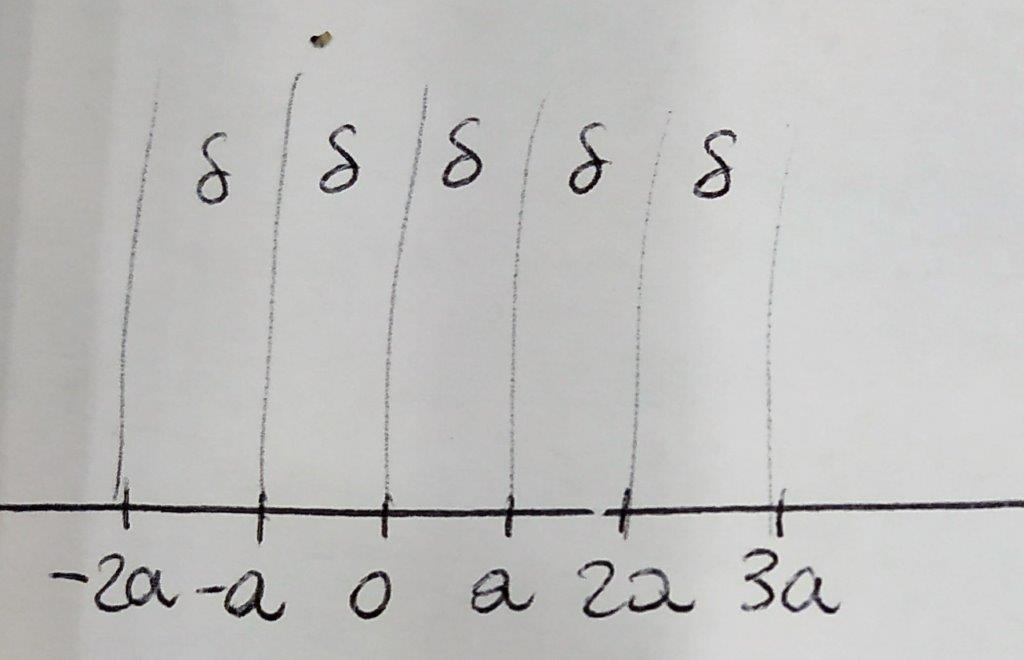
\includegraphics[scale=0.4]{Immagini/13_12/image001.jpg}
\caption{Grafico qualitativo del potenziale $V(x)$}
\end{figure}
\item Utilizzando il \textit{teorema di Bloch} e le condizioni di raccordo in $x_n = na$ per la funzione d'onda $\psi_\mathcal{E}$ e la sua derivata prima $\psi_\mathcal{E}'$, si determini l'equazione che collega il vettore d'onda $k$ di Bloch allo spettro $\sigma(H)$ dell'energia.
\item Si discuta qualitativamente la struttura di $\sigma(H)$ determinandone la degenerazione.
\item Si supponga ora che l'Hamiltoniana $H$ sia definita in $[0,Na] \subset \bb{R}$ (invece che su tutto $\bb{R}$), con $N \in \bb{N}$ e condizioni periodiche al bordo, restringendo la sommatoria $\sum_n$ nella definizione di $H$ a $n \in [0,N] \cap \bb{Z}$. Si discuta qualitativamente la struttura di $\sigma(H)$ in questo caso. 
\end{enumerate}
\begin{figure}[H]
\centering
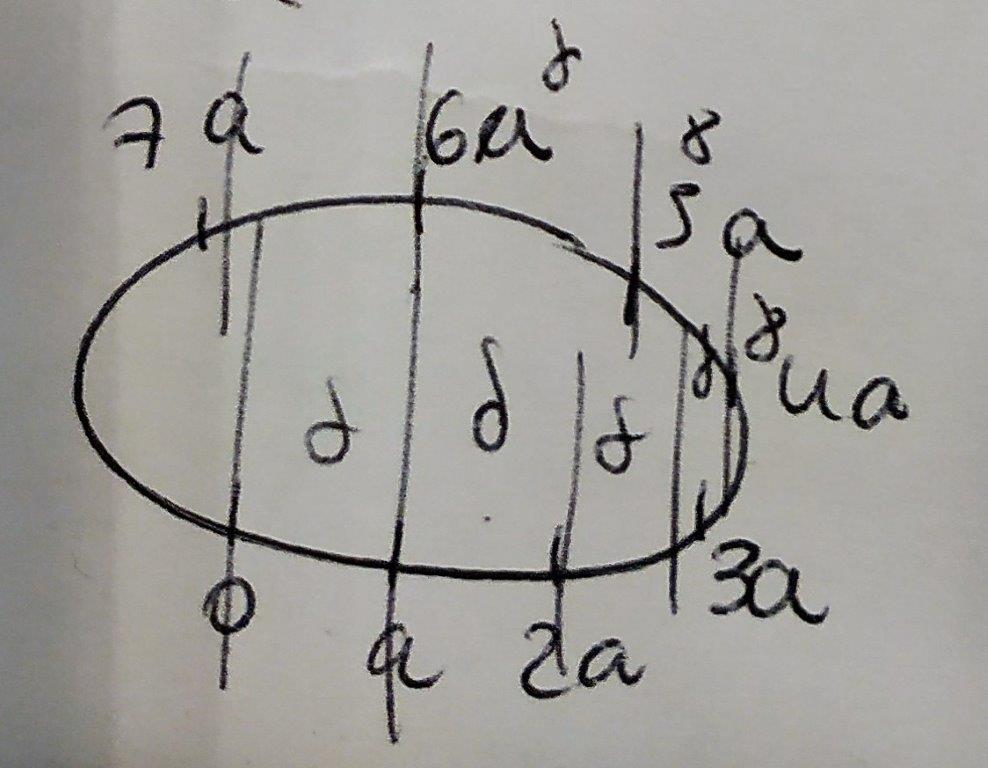
\includegraphics[scale=0.4]{Immagini/13_12/image002.jpg}
\caption{Schema qualitativo del potenziale \textit{con condizioni periodiche al bordo}}
\end{figure}


\subsection{Soluzione}
\begin{enumerate}
\item Partiamo scrivendo l'equazione di Schr\"odinger stazionaria:
\begin{align*}
-\frac{\hbar^2}{2m}\frac{d^2}{dx^2} \psi_\mathcal{E}(x) + V_0 \sum_{n\in \bb{Z}} \delta(x+na) \psi_\mathcal{E}(x) = \mathcal{E}\psi_\mathcal{E}(x)
\end{align*}
Seguendo il suggerimento, integriamola in un intervallo $\left[na-\frac{\xi}{2}, na+\frac{\xi}{2}\right]$:
\begin{align*}
&\int_{na-\frac{\xi}{2}}^{na+\frac{\xi}{2}} \hlc{Yellow}{-\frac{\hbar^2}{2m}\frac{d^2}{dx^2} \psi_\mathcal{E}(x)\, dx} + \int_{na-\frac{\xi}{2}}^{na+\frac{\xi}{2}} \hlc{SkyBlue}{V_0 \sum_{m\in \bb{Z}} \delta(x+ma)\psi_\mathcal{E}(x)\,dx} = \int_{na-\frac{\xi}{2}}^{na+\frac{\xi}{2}} \mathcal{E}\psi_\mathcal{E}(x) dx\\
\Rightarrow &\hlc{Yellow}{-\frac{\hbar^2}{2m}(\psi'_\mathcal{E}\left(na + \frac{\xi}{2}\right)-\psi_\mathcal{E}'\left(na-\frac{\xi}{2}\right)}
+\hlc{SkyBlue}{V_0 \psi_\mathcal{E}(na)} = \mathcal{E}\hlc{ForestGreen}{\int_{na-\frac{\xi}{2}}^{na+\frac{\xi}{2}} \psi_\mathcal{E}(x)\,dx}
\end{align*}
Prendendo il $\lim$ per $\xi \to 0$:
\begin{align}
-\frac{\hbar^2}{2m}\left(\psi_\mathcal{E}'(na^+)-\psi_\mathcal{E}'(na^-)\right) + V_0\psi_\mathcal{E}(na) = \hlc{ForestGreen}{0}
\label{eqn:raccordo_derivate}
\end{align}
Dove abbiamo usato la continuità di $\psi_\mathcal{E}(x)$ (data per ipotesi), per affermare che un suo integrale su un intervallo di misura nulla è nullo. La (\ref{eqn:raccordo_derivate}) così ottenuta è la relazione di raccordo, in forma implicita, per le derivate $\psi_\mathcal{E}'(x)$ in $x_n = na$.
\item Dal teorema di Bloch sappiamo che $\psi_\mathcal{E}(x)$ è \q{periodica a meno di una fase}. Infatti, vale $\psi_\mathcal{E}(x) = e^{ikx} u_{k,\mathcal{E}}(x)$, dove tale $u_{k,\mathcal{E}}(x)$ è una funzione periodica di periodo $a$. Perciò:
\begin{align}\nonumber
\psi_{\mathcal{E}}(x+na) &= e^{ik(x+na)}u_{k, \mathcal{E}}(x+na) \underset{(a)}{=} e^{ik(x+na)}u_{k,\mathcal{E}}(x)=\\
&\underset{(b)}{=} e^{ik(x+na)} e^{-ikx} \psi_\mathcal{E}(x) = e^{ikna}\psi_\mathcal{E}(x)
\label{eqn:periodicita_afase}
\end{align}
dove in (a) abbiamo usato la periodicità di $u_{k,\mathcal{E}}(x)$, e in (b) la definizione $u_{k,\mathcal{E}}(x) = e^{-ikx}\psi_\mathcal{E}(x)$.\\
Possiamo allora concentrarci sul trovare $\psi_\mathcal{E}(x)$ solo per $x \in [0,a]$, e usare la relazione (\ref{eqn:periodicita_afase}) e le condizioni di raccordo per trovare la $\psi_\mathcal{E}(x)$ per $x\in \bb{R}$. Date le $\psi_\mathcal{E}(x)$ conosciamo lo spettro $\sigma(H)$ (da cui sono indicizzate), che possiamo poi mettere in relazione a $k$.\\

Notiamo ora che per $x \in ]0,a[$ il potenziale $V(x) = 0$\marginpar{Autofunzioni $\psi_\mathcal{E}(x)$, $x \in ]0,a[$} è quello di una particella libera, di cui possiamo ricavare immediatamente le autofunzioni:
\begin{align}\nonumber
-\frac{\hbar^2}{2m}\psi_\mathcal{E}''(x) &=\mathcal{E}\psi_\mathcal{E}(x) \Rightarrow \psi_\mathcal{E}''(x) + \overbrace{\frac{2m\mathcal{E}}{\hbar^2}}^{q^2}\psi_\mathcal{E}(x) = 0\\
\Rightarrow \psi_\mathcal{E}(x) &= A e^{iqx} + Be^{-iqx} \quad q=\sqrt{\frac{2m\mathcal{E}}{\hbar^2}} \label{eqn:autofunzioni_periodiche}
\end{align}
dove $A, B \in \bb{C}$ dipendono dalle condizioni al contorno su $\psi_\mathcal{E}(x)$ e $\psi_\mathcal{E}'(x)$.\\
Partiamo esaminando quelle su $\psi_\mathcal{E}(x)$. Per trovarle, facciamo uso del teorema di Bloch. 
Sappiamo che $u_{\mathcal{E},k}(x) = e^{-ikx} \psi_\mathcal{E}(x)$ per Bloch è periodica di periodo $a$, ed è anche continua, dato che lo è $\psi_\mathcal{E}(x)$ per ipotesi. Perciò deve essere:
\begin{align}
u_{\mathcal{E},k}(0^-) = u_{\mathcal{E},k}(0^+)
\label{eqn:periodicita_uk}
\end{align}
La $\psi_\mathcal{E}(x)$ ricavata, tuttavia, vale solo in $]0,a[$, e mentre per $a^- \in ]0,a[$ non ci sono problemi, si ha $0^- \notin ]0,a[$, e quindi la (\ref{eqn:periodicita_uk}) non è immediatamente utilizzabile. Possiamo però \textit{aggirare il problema} usando la periodicità:
\begin{align}
\hlc{Yellow}{u_{\mathcal{E},k}(0^-)} = \hlc{SkyBlue}{u_{\mathcal{E},k}(a^-)} \Rightarrow e^{-ik0}\psi_\mathcal{E}(0) = e^{-ika}\psi_\mathcal{E}(a)
\label{eqn:periodic2}
\end{align}
Solo ora possiamo sostituire l'espressione trovata per $\psi_\mathcal{E}(x)$ in (\ref{eqn:autofunzioni_periodiche}) e trovare quindi la prima condizione di raccordo:\marginpar{Raccordo per $\psi_\mathcal{E}(x)$}
\begin{align}
\hlc{Yellow}{A + B }= \hlc{SkyBlue}{Ae^{i(q-k)a} + Be^{-i(q+k)a}}
\label{eqn:raccordo_func}
\end{align}
D'altro canto, l'equazione di raccordo per la derivata $\psi_\mathcal{E}'(x)$ è già stata ricavata in (\ref{eqn:raccordo_derivate}), e basta esplicitarla per $n=0$:
\begin{align*}
{\psi_\mathcal{E}'(0^+)} - \psi_\mathcal{E}'(0^-) = \frac{2mV_0}{\hbar^2}\psi_\mathcal{E}(0)
\end{align*}
Di nuovo notiamo che $0^- \notin [0,a]$, per cui dobbiamo usare la periodicità. Usando l'analoga di (\ref{eqn:periodic2}) per la derivata:
\begin{align*}
\psi_\mathcal{E}'(0^-) = e^{-ika} \psi_\mathcal{E}'(a^-)
\end{align*}
Otteniamo ora un'espressione in cui possiamo sostituire le derivate della $\psi_\mathcal{E}(x)$ trovata in (\ref{eqn:autofunzioni_periodiche}):\marginpar{Raccordo per $\psi'_\mathcal{E}(x)$}
\begin{align}\nonumber
\hlc{ForestGreen}{\psi'_\mathcal{E}(0^+)}-\hlc{Yellow}{e^{-ika}\psi'_\mathcal{E}(a^-)}&=\frac{2mV_0}{\hbar^2}\psi_\mathcal{E}(0)\\
\hlc{ForestGreen}{iq(A-B)} -\hlc{Yellow}{e^{-ika}iq(Ae^{iqa}-Be^{-iqa})} &= \frac{2mV_0}{\hbar^2}(A+B)
\label{eqn:raccordo_psiprima}
\end{align}
Infine, mettiamo a sistema le condizioni di raccordo per $\psi_\mathcal{E}(x)$ (\ref{eqn:raccordo_func}) e la derivata $\psi_\mathcal{E}'(x)$ (\ref{eqn:raccordo_psiprima}). Da questa troveremo la relazione cercata tra vettore di Bloch e spettro dell'energia.\\
\begin{align*}
\begin{cases}
A(1-e^{i(q-k)a}) +B(1-e^{-i(q+k)a})=0\\
A(iq)(1-e^{i(q-k)a})-B(iq)(1-e^{-i(q+k)a}) = \frac{2mV_0}{\hbar^2}(A+B)
\end{cases}
\end{align*}
Ponendo:
\begin{align*}
\hat{A}=(1-e^{i(q-k)a}); \quad \hat{B} = (1-e^{-i(q+k)a})
\end{align*}
Otteniamo:
\begin{align*}
\begin{cases}
A \hat{A} + B\hat{B}\\
iq(A\hat{A}-B\hat{B} = \frac{2mV_0}{\hbar^2}(A+B)
\end{cases}\Rightarrow 
\begin{cases}
B=-A\hat{A}/\hat{B}\\
\cancel{2}A\hat{A}(iq) = \frac{\cancel{2}mV_0}{\hbar^2}A\left(1-\frac{\hat{A}}{\hat{B}}\right)
\end{cases}
\end{align*}
Svolgendo i conti nella seconda equazione:
\begin{align*}
\hat{A}\hat{B}(iq) = \frac{mV_0}{\hbar^2}(\hat{B}-\hat{A})\\
\Rightarrow (iq)[1-e^{i(q-k)a}-e^{-i(q+k)a}+e^{-2ika}] = \frac{mV_0}{\hbar^2}(e^{i(q-k)a}-e^{-i(q+k)a})\span
\end{align*}
Moltiplicando entrambi i membri per $e^{ika}$ e dividendo per $2i$:
\begin{align*}
iq(e^{ika} + e^{-ika} - e^{iqa} - e^{-iqa})=\frac{mV_0}{\hbar^2} (e^{iqa}- e^{-iqa})\\
\Rightarrow q(\cos(ka)-\cos(qa)) = \frac{mV_0}{\hbar^2}\sin(qa)\span
\end{align*}
Poiché l'autovalore dell'energia è contenuto in $q$,\marginpar{$k(\mathcal{E})$} per trovare la relazione cercata basta ora isolare il termine con $k$:
\begin{align}
\cos(ka) = \cos(qa) + \frac{mV_0}{\hbar^2} \frac{\sin(qa)}{q} \quad q=\sqrt{\frac{2m\mathcal{E}}{\hbar^2}}
\label{eqn:bloch-energia-relation}
\end{align}
\item Com'è fatto, qualitativamente, lo spettro $\sigma(H)$, e qual è la sua degenerazione?\\
Partiamo da (\ref{eqn:bloch-energia-relation}), dove imponiamo che (dal teorema di Bloch) $k \in \left[-\frac{\pi}{a}, \frac{\pi}{a}\right]$, da cui $-1 \leq \cos(ka)\leq +1$, e perciò:
\begin{align*}
-1 \leq \underbrace{\cos(qa) + \frac{mV_0}{\hbar^2} \frac{\sin(qa)}{q}}_{y(q)}\leq 1
\end{align*} 
Si ha allora che non tutti i valori di $q(\mathcal{E})$ sono, a priori, permessi, ma solo quelli per cui $-1 < y(q) < +1$, come rappresentato in figura \ref{fig:bande}.

\begin{figure}[H]
\centering
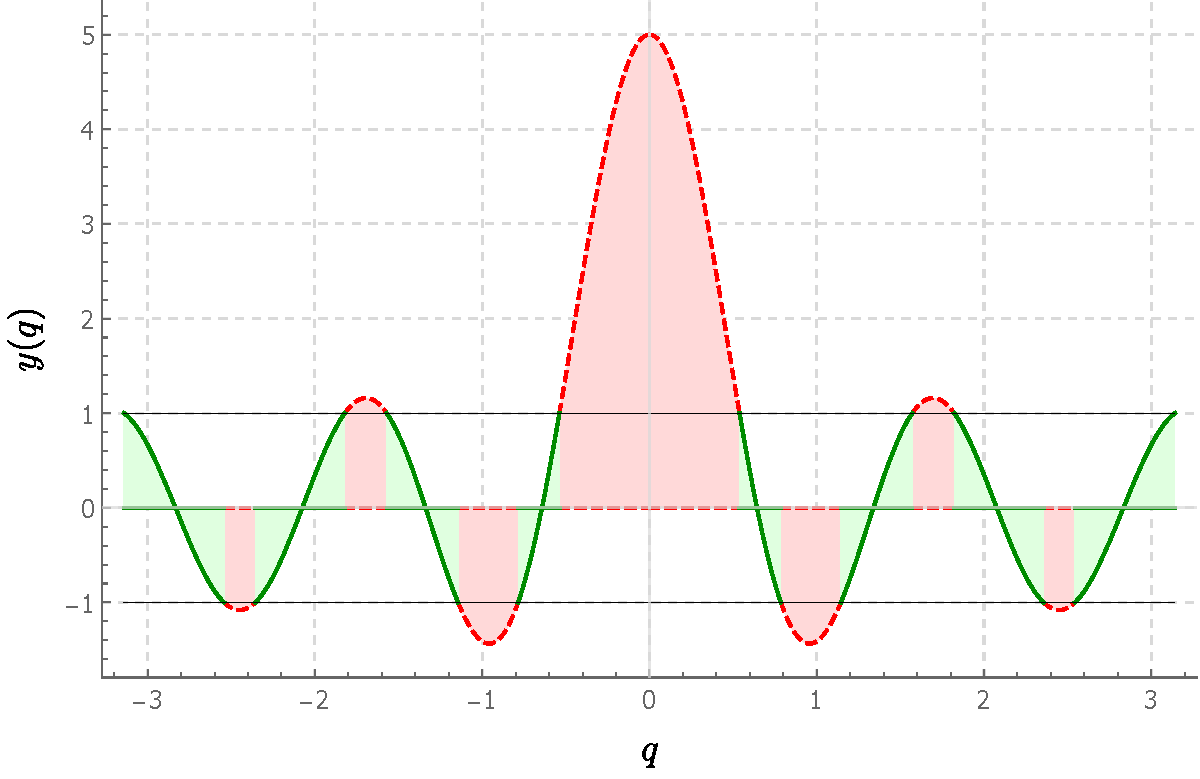
\includegraphics[width=0.8\textwidth]{Immagini/13_12/plot1.pdf}
\caption{Spettro a bande: solo i valori di $q(\mathcal{E})$ evidenziati in verde sono fisicamente permessi (per $mV_0/\hbar^2=1$, $a=4$)\label{fig:bande}}
\end{figure}
Escludiamo le regioni in cui la funzione esce dal range $-1 \leq y \leq +1$.\\

Per le $q$ ammesse\marginpar{Spettro continuo a bande}, la $\psi_\mathcal{E}(x)$ non sta in $L^2$ (oscilla all'infinito), e perciò $\sigma(H)$ è continuo. Il supporto di $\sigma(H)$ è l'unione di intervalli disgiunti
che chiameremo \textit{bande} (i tratti evidenziati in verde sull'asse $x$ del grafico \ref{fig:bande}).\\
Quanti modi sono possibili a energia fissata?\marginpar{Degenerazione di $\sigma(H)$} Notiamo che $\sigma(H)$ dipende univocamente da $q$. Fissare l'energia significa impostare:
\begin{align*}
\mathcal{E} = \frac{\hbar^2 q^2}{2m}
\end{align*}
e per una certa $\mathcal{E}$ sono possibili $2$ valori di $q$: $q$ e $-q$. Perciò la degenerazione di $\sigma(H)$ è $2$.
\item Consideriamo ora lo stesso sistema confinato in una regione finita, con $x \in [0,Na]$. Dalle condizioni al contorno periodiche per la funzione d'onda $\psi_\mathcal{E}(x)$:
\begin{align*}
\psi_\mathcal{E}(0) = \psi_\mathcal{E}(Na) \underset{(a)}{=} e^{ikNa}\psi_\mathcal{E}(0) \Rightarrow e^{ikNa} = 1
\end{align*}
dove in (a) si è applicato il teorema di Bloch. Si ha perciò una condizione ulteriore sull'esponente $kNa$:
\begin{align*}
kNa \in 2\pi\bb{Z} \Rightarrow  k \in \frac{2\pi \bb{Z}}{Na}\cap \left[-\frac{\pi}{a}, \frac{\pi}{a}\right]
\end{align*}
Ne segue che $k$ può assumere solo valori in un set discreto e finito. Poiché $k$ è legato a $\sigma(H)$ come visto al punto precedente, ricaviamo che in questo caso l'energia ha uno \textit{spettro discreto}. Infatti, la $\psi_\mathcal{E}(x)$ è ora ristretta a un intervallo compatto, e perciò non \q{oscilla più all'infinito}: è quindi modulo-quadro sommabile e si trova in $L^2$:
\begin{align*}
\psi_\mathcal{E}(x) \in L^2([0,Na],dx) \Rightarrow \sigma(H) \text{ è discreto}
\end{align*}
E in effetti:
\begin{align*}
\left\{k | k \in \frac{2\pi\bb{Z}}{Na} \cap \left[-\frac{\pi}{a}, \frac{\pi}{a}\right] \right\} \text{ è discreto}
\end{align*}
Perciò nelle \textit{bande} di figura \ref{fig:bande} solo alcuni valori \textit{discreti}\marginpar{Spettro discreto a bande} sono ammessi: invece di avere tratti evidenziati \q{continui} per i $q$ ammessi si ha una sequenza di \textit{singoli punti} (seppur molto fini, dato che ogni banda può contenere un numero di stati dell'ordine di $10^{23}$) . Chiamiamo questo tipo di spettro uno \textit{spettro discreto a bande}: si hanno quindi intervalli \q{larghi} che contengono un gran numero di autovalori molto vicini tra loro, separati da \textit{gap} in cui non ve ne è nessuno.
\end{enumerate}

L'esercizio appena fatto ha un'utile interpretazione fisica, in quanto costituisce un \textit{toy model} (modello semplificato) per un cristallo 1D.\marginpar{Cristalli in $d=1$}\\
Consideriamo una \textit{fila} di atomi \textit{equispaziati}. Ciascuno di essi ha un potenziale coulombiano, e avremo degli stati discreti corrispondenti agli stati legati degli elettroni (i \q{consueti} orbitali). Un elettrone può, per \textit{effetto tunnel}, attraversare lo spazio tra un atomo e l'altro, schematizzabile come una barriera (le $\delta$ nell'esempio appena fatto). Se il cristallo è infinito, la funzione d'onda che incorpora tutte le \textit{onde evanescenti} di trasferimento da un atomo all'altro \textit{non} appartiene a $L^2$. \textit{Fisicamente}, ciò significa che gli elettroni possono \textit{spostarsi arbitrariamente lontano}. Tali stati costituiscono \q{un'onda}.\\
In un reticolo periodico, l'elettrone si comporta perciò \q{come un'onda}, da cui lo \textit{spettro continuo a bande}.\\
\begin{figure}[H]
\centering
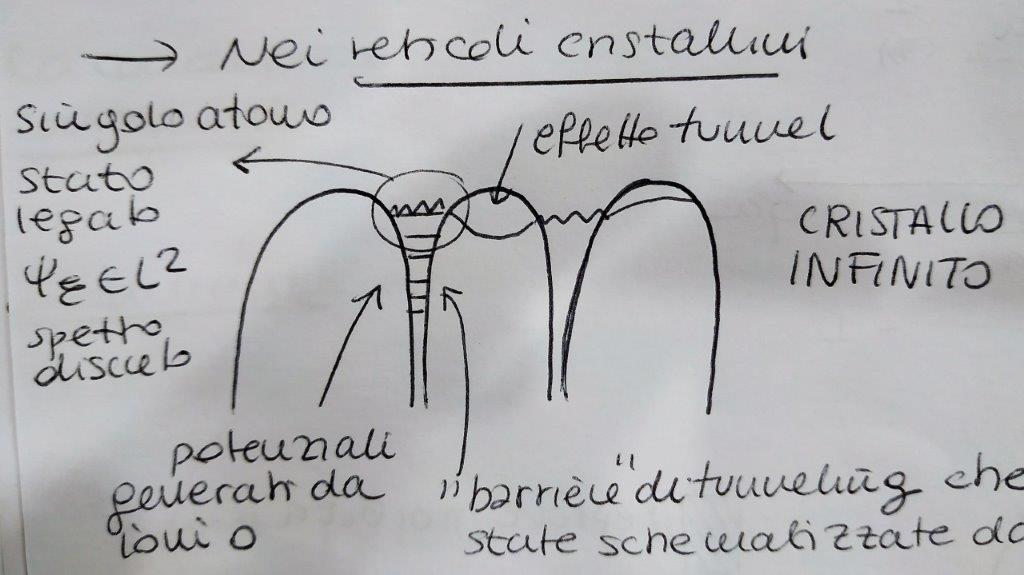
\includegraphics[scale=0.4]{Immagini/13_12/image004.jpg}
\caption{La possibilità degli elettroni di passare da un atomo all'altro del reticolo cristallino per \textit{effetto tunnel} fa sì che $\sigma(H)$ sia continuo}
\end{figure}
Se il cristallo è finito, avremo invece uno \textit{spettro discreto a bande}.\\
In un \textit{reticolo ionico} con $N_e$ elettroni, l'Hamiltoniana delle particelle singole è data da:
\begin{align*}
H_i = \frac{P_i^2}{2m} + V(x_i)
\end{align*}
con $P_i, X_i$ dell'elettrone $i$-esimo.\\
L'Hamiltoniana del sistema composto è data, ignorando le interazioni tra i vari elettroni:
\begin{align*}
H \approx \sum_{i=1}^{N_e} H_i
\end{align*}
\textbf{Nota}: $H$ è simmetrica per scambio di variabili, come vogliamo dato che gli elettroni sono indistinguibili.\\

Per il principio di esclusione di Pauli, due elettroni non possono avere gli stessi valori per un ICOC di particella singola, che in questo caso è dato da $\{q\}$:
\begin{align*}
q = \pm \sqrt{\frac{2mH}{\hbar^2}}
\end{align*}
Gli elettroni prendono i vari $q$ possibili, \textit{dal basso verso l'alto}. Dato che $N_e$ è finito, si ha, come diretta conseguenza del principio di Pauli, che esiste un $q_{max} \equiv q_F$, detto \textbf{momento di Fermi}.\index{Momento di Fermi}\marginpar{Momento di Fermi}\\
%Inserire plot
%(Nota: i punti di una banda sono molto fitti, dato che sono dell'ordine di $N_e \sim 10^{23}$.\\
Avremo allora due possibilità:
\begin{itemize}
\item $q_F$ sta all'interno della banda \textit{permessa}. Se allora applichiamo una differenza di potenziale, l'energia (cinetica media) degli elettroni \textit{aumenta}. Dato che esistono $q$ di energia permessa sopra a $q_F$, gli elettroni possono occuparli, e quindi spostarsi. Tale processo descrive la \textit{conduzione} nei metalli.
\item Se invece $q_F$ sta alla \textit{fine} della banda permessa (ossia tutti i valori permessi sono \textit{pieni}), anche applicando una differenza di potenziale gli elettroni non possono muoversi, dato che non hanno livelli energetici \textit{permessi} subito sopra che possano occupare. Questo è la descrizione dei materiali \textit{isolanti}.
\end{itemize}

L'idea alla base dell'elettronica è quella di trovare un \textit{gap} tra due bande che sia \textit{sufficientemente piccolo} in modo da poter essere superato applicando un opportuno potenziale, ma \textit{sufficientemente alto} affinché l'agitazione termica non basti a far ciò.\\
Perciò il funzionamento dell'elettronica è un altro esempio di applicazione del principio di esclusione di Pauli.


\end{document}

